\documentclass[12pt,a4paper]{article}
\usepackage[a4paper, margin=0.8in, headheight=14pt]{geometry}
\usepackage{fontspec}
\usepackage{unicode-math}
\setmainfont{TeX Gyre Pagella}
\setmonofont[Scale=0.88]{TeX Gyre Cursor}
\setmathfont{Latin Modern Math}

\usepackage{xcolor}
\usepackage{colortbl}
\usepackage{titlesec}
\usepackage{enumitem}
\usepackage{tabularx}
\usepackage{booktabs}
\usepackage{array}
\usepackage{amsmath}
\allowdisplaybreaks
\usepackage{tikz}
\usetikzlibrary{shapes.geometric, arrows.meta, positioning, calc, fit, decorations.pathreplacing, patterns}
\usepackage{tcolorbox}
\tcbuselibrary{skins, breakable}
\usepackage{hyperref}
\usepackage{fancyhdr}
\usepackage{graphicx}
\usepackage{microtype}
\hyphenpenalty=10000
\exhyphenpenalty=10000
\sloppy
\usepackage{caption}
\usepackage{setspace}
\usepackage{multirow}
\usepackage{tocloft}

% ─── Q&A helper ────────────────────────────────────────────────────────────────
\newcommand{\Q}[1]{\textbf{#1}\par\noindent\ignorespaces}

% ─── Colour Palette ────────────────────────────────────────────────────────────
\definecolor{myred}{RGB}{196,30,58}
\definecolor{mydark}{RGB}{30,30,50}
\definecolor{mygreen}{RGB}{14,120,80}
\definecolor{myteal}{RGB}{0,130,140}
\definecolor{myamber}{RGB}{220,130,20}
\definecolor{mypurple}{RGB}{90,40,140}
\definecolor{mygray}{RGB}{248,249,251}
\definecolor{mgframe}{RGB}{215,220,230}
\definecolor{watermark}{RGB}{145,150,170}
\definecolor{hdrred}{RGB}{250,232,235}
\definecolor{hdrgreen}{RGB}{220,244,233}
\definecolor{hdrteal}{RGB}{220,242,244}
\definecolor{hdramber}{RGB}{253,242,215}
\definecolor{hdrpurple}{RGB}{238,228,255}
\definecolor{hdrgray}{RGB}{238,240,245}
\definecolor{rowalt}{RGB}{250,251,253}

% ─── Section Formatting ────────────────────────────────────────────────────────
\titleformat{\section}
  {\large\bfseries\color{myred}}{\thesection.}{0.5em}{}
  [\vspace{1pt}{\color{myred}\rule{\linewidth}{0.8pt}}]
\titleformat{\subsection}
  {\normalsize\bfseries\color{myteal}}{\thesubsection}{0.5em}{}
\titlespacing*{\section}{0pt}{18pt}{7pt}
\titlespacing*{\subsection}{0pt}{11pt}{4pt}

% ─── Paragraph ─────────────────────────────────────────────────────────────────
\setlength{\parindent}{0pt}
\setlength{\parskip}{4pt}

% ─── TOC Styling ───────────────────────────────────────────────────────────────
\renewcommand{\cfttoctitlefont}{\large\bfseries\color{myred}}
\renewcommand{\cftaftertoctitle}{\par\noindent{\color{myred}\rule{\linewidth}{0.8pt}}}
\setlength{\cftbeforetoctitleskip}{0pt}
\setlength{\cftaftertoctitleskip}{6pt}
\renewcommand{\cftsecfont}{\normalsize\bfseries\color{mydark}}
\renewcommand{\cftsecpagefont}{\normalsize\bfseries\color{mydark}}
\renewcommand{\cftsecleader}{\cftdotfill{\cftdotsep}}
\setlength{\cftbeforesecskip}{7pt}
\renewcommand{\cftsubsecfont}{\small\color{mydark}}
\renewcommand{\cftsubsecpagefont}{\small\color{mydark}}
\setlength{\cftbeforesubsecskip}{3pt}
\setlength{\cftsubsecindent}{1.4em}

% ─── Table helpers ─────────────────────────────────────────────────────────────
\renewcommand{\arraystretch}{1.45}
\setlength{\tabcolsep}{6pt}
\arrayrulecolor{mydark}
\newcolumntype{B}[1]{>{\small\bfseries\raggedright\arraybackslash}m{#1}}
\newcolumntype{Y}{>{\small\raggedright\arraybackslash}X}
\renewcommand{\tabularxcolumn}[1]{m{#1}}

% ─── Header / Footer ───────────────────────────────────────────────────────────
\pagestyle{fancy}
\fancyhf{}
\fancyhead[L]{\small\color{myred}\textbf{EC303}\;\color{mydark}--- Signals and System}
\fancyhead[R]{\small\color{myteal}\textbf{Module 2 Notes}}
\fancyfoot[C]{\small\color{mydark}\thepage}
\fancyfoot[R]{\small\color{watermark}\textit{\copyright\ Biraj}}
\renewcommand{\headrulewidth}{0.5pt}
\renewcommand{\footrulewidth}{0.3pt}

% ─── Hyperref ──────────────────────────────────────────────────────────────────
\hypersetup{
  colorlinks=true, linkcolor=myteal, urlcolor=myteal,
  pdfauthor={Biraj Sarkar (CGEC)},
  pdftitle={EC303 --- Module 2 Notes: Linear Shift-Invariant Systems}
}

% ─── tcolorbox styles ──────────────────────────────────────────────────────────
\tcbset{
  tikzbox/.style={
    colback=mygray, colframe=mgframe, boxrule=0.6pt, arc=4pt,
    left=8pt, right=8pt, top=6pt, bottom=6pt,
    colbacktitle=mgframe, coltitle=mydark,
    fonttitle=\small\bfseries
  },
  defbox/.style={
    colback=hdrgreen, colframe=mygreen, boxrule=0.8pt, arc=4pt,
    left=9pt, right=9pt, top=6pt, bottom=6pt,
    colbacktitle=mygreen, coltitle=white,
    fonttitle=\small\bfseries
  },
  formulabox/.style={
    colback=hdrteal, colframe=myteal, boxrule=0.8pt, arc=4pt,
    left=9pt, right=9pt, top=6pt, bottom=6pt,
    colbacktitle=myteal, coltitle=white,
    fonttitle=\small\bfseries
  },
  examplebox/.style={
    colback=hdramber, colframe=myamber, boxrule=0.8pt, arc=4pt,
    left=9pt, right=9pt, top=6pt, bottom=6pt,
    colbacktitle=myamber, coltitle=white,
    fonttitle=\small\bfseries
  },
  masonbox/.style={
    colback=hdrpurple, colframe=mypurple, boxrule=0.8pt, arc=4pt,
    left=9pt, right=9pt, top=6pt, bottom=6pt,
    colbacktitle=mypurple, coltitle=white,
    fonttitle=\small\bfseries
  },
  exambox/.style={
    colback=hdrpurple, colframe=mypurple, boxrule=1pt, arc=5pt,
    left=10pt, right=10pt, top=8pt, bottom=8pt,
    colbacktitle=mypurple, coltitle=white,
    fonttitle=\bfseries,
    breakable, title after break={\textbf{Frequently Asked / Viva Questions (contd.)}}
  }
}

\tcbset{breakable}
\tcbset{after={\color{black}}}

% ─── TikZ Global Styles ────────────────────────────────────────────────────────
\tikzset{
  sysblock/.style={draw=myteal, fill=hdrteal, thick, rectangle, rounded corners=3pt, minimum height=1cm, minimum width=2.4cm, align=center, font=\small\bfseries},
  circnode/.style={draw=myred, fill=hdrred, circle, thick, inner sep=1.5pt, font=\small\bfseries},
  arrowline/.style={-{Latex[length=2.5mm]}, thick, color=mydark},
  dashline/.style={thick, dashed, color=myteal}
}

% ─── Document ──────────────────────────────────────────────────────────────────
\begin{document}

% ─── Title Block ───────────────────────────────────────────────────────────────
\begin{center}
  {\Large\bfseries\color{myred} EC303 --- Signals and System}\\[4pt]
  {\large\bfseries\color{mydark} Module 2: Linear Shift-Invariant (LSI) Systems \& Convolution}\\[3pt]
  {\small\color{watermark} Prepared by \textbf{Biraj Sarkar (CGEC)} $\cdot$ MAKAUT B.Tech ECE (2023--27)}\\[2pt]
  {\small\color{watermark} Authoritative Syllabus-Aligned Notes}
\end{center}
\vspace{-4pt}
\noindent{\color{myred}\rule{\linewidth}{1.2pt}}

% ─── Table of Contents ─────────────────────────────────────────────────────────
\tableofcontents
\vspace{10pt}
\noindent{\color{mgframe}\rule{\linewidth}{0.6pt}}

% ───────────────────────────────────────────────────────────────────────────────
\section{Linear Shift-Invariant (LSI) Systems Overview}
% ───────────────────────────────────────────────────────────────────────────────

\begin{tcolorbox}[defbox, title={\textbf{Definition: Linear Shift-Invariant (LSI / LTI) System}}]
A system $\mathcal{T}$ is called a \textbf{Linear Shift-Invariant (LSI)} or \textbf{Linear Time-Invariant (LTI)} system if it satisfies both the principle of \textbf{Linearity} (superposition: additivity and homogeneity) and the condition of \textbf{Shift-Invariance} (time-invariance).

Formally, for arbitrary scalar multipliers $a, b \in \mathbb{C}$ and arbitrary inputs $x_1(t), x_2(t)$:
\begin{enumerate}[topsep=2pt, itemsep=2pt]
  \item \textbf{Superposition (Linearity):} $\mathcal{T}\{a x_1(t) + b x_2(t)\} = a \mathcal{T}\{x_1(t)\} + b \mathcal{T}\{x_2(t)\} = a y_1(t) + b y_2(t)$.
  \item \textbf{Shift-Invariance (Time-Invariance):} If $\mathcal{T}\{x(t)\} = y(t)$, then $\mathcal{T}\{x(t - t_0)\} = y(t - t_0)$ for any arbitrary shift $t_0 \in \mathbb{R}$ (or $n_0 \in \mathbb{Z}$ in discrete-time).
\end{enumerate}
\end{tcolorbox}

\subsection{Representation of Signals Through Shifted Impulses}
Any continuous-time signal $x(t)$ can be viewed as a continuum of weighted, shifted Dirac delta impulses via the sifting property:
\begin{equation}
  x(t) = \int_{-\infty}^{\infty} x(\tau) \delta(t - \tau) d\tau
\end{equation}
Similarly, any discrete-time signal $x[n]$ is exactly decomposed into a linear combination of weighted, shifted Kronecker deltas:
\begin{equation}
  x[n] = \sum_{k=-\infty}^{\infty} x[k] \delta[n - k]
\end{equation}
This decomposition forms the conceptual bedrock of LTI system analysis: because the system is linear and time-invariant, knowledge of its response to a single unit impulse ($\delta(t)$ or $\delta[n]$) is sufficient to completely determine its response to \textit{any arbitrary} input signal.

% ───────────────────────────────────────────────────────────────────────────────
\section{Impulse Response and Step Response}
% ───────────────────────────────────────────────────────────────────────────────

\subsection{The Impulse Response $h(t)$ and $h[n]$}

\begin{tcolorbox}[defbox, title={\textbf{Definition: Impulse Response}}]
The \textbf{Impulse Response} $h(t)$ (in CT) or $h[n]$ (in DT) is the output of an LSI system when the input is a unit impulse applied at the origin under initial rest conditions (zero energy stored in the system):
\begin{align}
  h(t) &\triangleq \mathcal{T}\{\delta(t)\} \quad \text{(Continuous-Time)} \\
  h[n] &\triangleq \mathcal{T}\{\delta[n]\} \quad \text{(Discrete-Time)}
\end{align}
\end{tcolorbox}

\textbf{Physical Significance:}
\begin{itemize}[topsep=2pt, itemsep=2pt]
  \item It acts as the ``fingerprint'' or signature of an LSI system. Every structural attribute—memory, causality, stability, invertibility, and frequency selectivity—is entirely encoded in $h(t)$ or $h[n]$.
  \item It characterizes the transient relaxation dynamics of the physical system following an instantaneous excitation.
\end{itemize}

\subsection{The Step Response $s(t)$ and $s[n]$}

\begin{tcolorbox}[defbox, title={\textbf{Definition: Step Response}}]
The \textbf{Step Response} $s(t)$ (in CT) or $s[n]$ (in DT) is the system output when excited by a unit step function $u(t)$ or $u[n]$ under zero initial state:
\begin{equation}
  s(t) \triangleq \mathcal{T}\{u(t)\}, \qquad s[n] \triangleq \mathcal{T}\{u[n]\}
\end{equation}
\end{tcolorbox}

\subsection{Relationship Between Impulse Response and Step Response}
Since the unit step is the integral (running sum) of the unit impulse:
\begin{equation}
  u(t) = \int_{-\infty}^t \delta(\tau) d\tau, \qquad u[n] = \sum_{k=-\infty}^n \delta[k]
\end{equation}
By linearity and time-invariance, the step response is the running integral (or running sum) of the impulse response:

\begin{tcolorbox}[formulabox, title={\textbf{Fundamental Inter-relationships: Impulse $\leftrightarrow$ Step Response}}]
\textbf{Continuous-Time (CT):}
\begin{equation}
  s(t) = \int_{-\infty}^{t} h(\tau) d\tau \iff h(t) = \frac{ds(t)}{dt}
\end{equation}
\textbf{Discrete-Time (DT):}
\begin{equation}
  s[n] = \sum_{k=-\infty}^{n} h[k] \iff h[n] = s[n] - s[n-1] = \nabla s[n]
\end{equation}
where $\nabla$ denotes the backward difference operator.
\end{tcolorbox}

\begin{tcolorbox}[examplebox, title={\textbf{Derivation Example: Step Response of First-Order RC Circuit}}]
Consider a simple low-pass RC series circuit where input $x(t) = v_{in}(t)$ and output $y(t) = v_C(t)$. The differential equation is $RC \frac{dy(t)}{dt} + y(t) = x(t)$.
\begin{enumerate}[topsep=2pt, itemsep=2pt]
  \item The impulse response is obtained by setting $x(t) = \delta(t)$:
  \begin{equation*}
    h(t) = \frac{1}{RC} e^{-t/RC} u(t)
  \end{equation*}
  \item The step response $s(t)$ is calculated via running integration for $t \ge 0$:
  \begin{equation*}
    s(t) = \int_0^t \frac{1}{RC} e^{-\tau/RC} d\tau = \left[ -e^{-\tau/RC} \right]_0^t = \left( 1 - e^{-t/RC} \right) u(t)
  \end{equation*}
  \item Differentiating $s(t)$ recovers $h(t)$:
  \begin{equation*}
    \frac{ds(t)}{dt} = \frac{1}{RC} e^{-t/RC} u(t) + (1 - e^{-t/RC}) \delta(t) = \frac{1}{RC} e^{-t/RC} u(t) + 0 = h(t) \quad \text{(since } 1-e^0 = 0\text{)}.
  \end{equation*}
\end{enumerate}
\end{tcolorbox}

% ───────────────────────────────────────────────────────────────────────────────
\section{The Convolution Operation}
% ───────────────────────────────────────────────────────────────────────────────

\subsection{Derivation of the Convolution Integral (CT)}
Let a continuous-time LSI system $\mathcal{T}$ have impulse response $h(t) = \mathcal{T}\{\delta(t)\}$.
\begin{enumerate}[topsep=2pt, itemsep=2pt]
  \item Express the input $x(t)$ using the sifting property:
  \begin{equation}
    x(t) = \int_{-\infty}^{\infty} x(\tau) \delta(t - \tau) d\tau
  \end{equation}
  \item Apply the transformation $\mathcal{T}$ to both sides:
  \begin{equation}
    y(t) = \mathcal{T}\{x(t)\} = \mathcal{T}\left\{ \int_{-\infty}^{\infty} x(\tau) \delta(t - \tau) d\tau \right\}
  \end{equation}
  \item By linearity (additivity over continuum and homogeneity for scalar $x(\tau)$):
  \begin{equation}
    y(t) = \int_{-\infty}^{\infty} x(\tau) \mathcal{T}\{\delta(t - \tau)\} d\tau
  \end{equation}
  \item By shift-invariance, $\mathcal{T}\{\delta(t - \tau)\} = h(t - \tau)$:
  \begin{equation}
    y(t) = \int_{-\infty}^{\infty} x(\tau) h(t - \tau) d\tau \triangleq x(t) * h(t)
  \end{equation}
\end{enumerate}

\subsection{Derivation of the Convolution Sum (DT)}
Similarly, for a discrete-time LSI system where $h[n] = \mathcal{T}\{\delta[n]\}$:
\begin{align}
  x[n] &= \sum_{k=-\infty}^{\infty} x[k] \delta[n - k] \\
  y[n] &= \mathcal{T}\{x[n]\} = \sum_{k=-\infty}^{\infty} x[k] \mathcal{T}\{\delta[n - k]\} = \sum_{k=-\infty}^{\infty} x[k] h[n - k] \triangleq x[n] * h[n]
\end{align}

\begin{tcolorbox}[formulabox, title={\textbf{Core Formulation: Convolution Integral and Sum}}]
\begin{align}
  y(t) &= x(t) * h(t) = \int_{-\infty}^{\infty} x(\tau) h(t - \tau) d\tau = \int_{-\infty}^{\infty} h(\tau) x(t - \tau) d\tau \\
  y[n] &= x[n] * h[n] = \sum_{k=-\infty}^{\infty} x[k] h[n - k] = \sum_{k=-\infty}^{\infty} h[k] x[n - k]
\end{align}
\end{tcolorbox}

\subsection{Graphical Interpretation of Convolution}
Evaluating convolution graphically consists of four rigorous sequential steps:
\begin{enumerate}[topsep=2pt, itemsep=3pt]
  \item \textbf{Change of Variable:} Plot $x(\tau)$ and $h(\tau)$ as functions of the dummy variable $\tau$.
  \item \textbf{Folding (Time Reversal):} Flip $h(\tau)$ about the vertical axis to obtain $h(-\tau)$.
  \item \textbf{Shifting (Time Delay):} Shift $h(-\tau)$ by time $t$ to obtain $h(t - \tau)$ (right-shift for $t > 0$, left-shift for $t < 0$).
  \item \textbf{Multiplication and Integration/Summation:} Multiply $x(\tau)$ and $h(t - \tau)$ pointwise, and evaluate the area under the product curve over the overlapping support interval.
\end{enumerate}

\begin{tcolorbox}[tikzbox, title={\textbf{TikZ Illustration: Graphical Convolution Mechanism}}]
\begin{center}
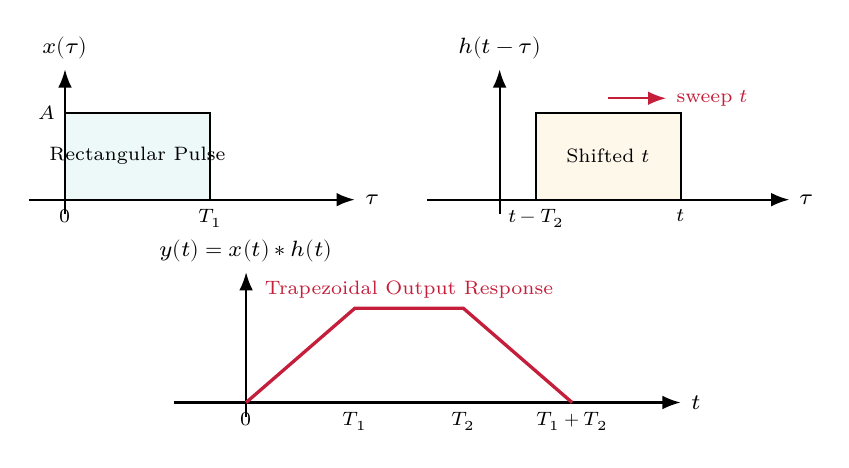
\begin{tikzpicture}[>=Latex, scale=0.92]
  % Step 1: Input x(tau)
  \draw[->, thick] (-0.5,0) -- (4,0) node[right] {\footnotesize $\tau$};
  \draw[->, thick] (0,-0.2) -- (0,1.8) node[above] {\footnotesize $x(\tau)$};
  \draw[thick, fill=hdrteal, fill opacity=0.5] (0,0) -- (0,1.2) -- (2,1.2) -- (2,0) -- cycle;
  \node at (1,0.6) {\scriptsize Rectangular Pulse};
  \node[below] at (0,0) {\scriptsize $0$};
  \node[below] at (2,0) {\scriptsize $T_1$};
  \node[left] at (0,1.2) {\scriptsize $A$};

  % Step 2: Folded and Shifted h(t - tau)
  \begin{scope}[xshift=6cm]
    \draw[->, thick] (-1,0) -- (4,0) node[right] {\footnotesize $\tau$};
    \draw[->, thick] (0,-0.2) -- (0,1.8) node[above] {\footnotesize $h(t-\tau)$};
    \draw[thick, fill=hdramber, fill opacity=0.5] (0.5,0) -- (0.5,1.2) -- (2.5,1.2) -- (2.5,0) -- cycle;
    \node at (1.5,0.6) {\scriptsize Shifted $t$};
    \node[below] at (0.5,0) {\scriptsize $t - T_2$};
    \node[below] at (2.5,0) {\scriptsize $t$};
    \draw[->, myred, thick] (1.5,1.4) -- (2.3,1.4) node[right, myred] {\scriptsize sweep $t$};
  \end{scope}

  % Step 3: Overlap & Output
  \begin{scope}[yshift=-2.8cm, xshift=2.5cm]
    \draw[->, thick] (-1,0) -- (6,0) node[right] {\footnotesize $t$};
    \draw[->, thick] (0,-0.2) -- (0,1.8) node[above] {\footnotesize $y(t) = x(t)*h(t)$};
    \draw[very thick, myred] (0,0) -- (1.5,1.3) -- (3.0,1.3) -- (4.5,0);
    \node[below] at (0,0) {\scriptsize $0$};
    \node[below] at (1.5,0) {\scriptsize $T_1$};
    \node[below] at (3.0,0) {\scriptsize $T_2$};
    \node[below] at (4.5,0) {\scriptsize $T_1+T_2$};
    \node[above, myred] at (2.25,1.3) {\scriptsize Trapezoidal Output Response};
  \end{scope}
\end{tikzpicture}
\end{center}
\end{tcolorbox}

\subsection{Properties of Convolution}

\par\vspace{6pt}\noindent
\begingroup
\setlength{\tabcolsep}{5pt}
\setlength{\extrarowheight}{3pt}
\renewcommand{\arraystretch}{1.4}
\begin{tabularx}{\linewidth}{|B{3.8cm}|Y|Y|}
\hline
\textbf{Property} & \textbf{Continuous-Time Formulation} & \textbf{Discrete-Time Formulation} \\
\hline
Commutative & $x(t) * h(t) = h(t) * x(t)$ & $x[n] * h[n] = h[n] * x[n]$ \\
\hline
Associative & $[x(t) * h_1(t)] * h_2(t) = x(t) * [h_1(t) * h_2(t)]$ & $[x[n] * h_1[n]] * h_2[n] = x[n] * [h_1[n] * h_2[n]]$ \\
\hline
Distributive & $x(t) * [h_1(t) + h_2(t)] = x * h_1 + x * h_2$ & $x[n] * [h_1[n] + h_2[n]] = x * h_1 + x * h_2$ \\
\hline
Shift Property & $x(t - t_1) * h(t - t_2) = y(t - t_1 - t_2)$ & $x[n - n_1] * h[n - n_2] = y[n - n_1 - n_2]$ \\
\hline
Identity Element & $x(t) * \delta(t) = x(t)$ & $x[n] * \delta[n] = x[n]$ \\
\hline
Derivative Property & $\frac{d}{dt}[x(t) * h(t)] = \frac{dx(t)}{dt} * h(t) = x(t) * \frac{dh(t)}{dt}$ & $\nabla[x[n] * h[n]] = \nabla x[n] * h[n] = x[n] * \nabla h[n]$ \\
\hline
Duration Property & If lengths are $L_1$ and $L_2$, duration of $y(t)$ is $L_1 + L_2$. & Number of non-zero samples is $N_1 + N_2 - 1$. \\
\hline
\end{tabularx}
\endgroup

\subsection{Interconnection of LSI Systems}
\begin{itemize}[topsep=2pt, itemsep=3pt]
  \item \textbf{Cascade (Series) Connection:} Equivalent impulse response is the convolution of individual impulse responses:
  \begin{equation}
    h_{eq}(t) = h_1(t) * h_2(t) = h_2(t) * h_1(t)
  \end{equation}
  By the commutative property, the order of cascaded LSI subsystems can be interchanged without altering the overall response.
  \item \textbf{Parallel Connection:} Equivalent impulse response is the arithmetic sum of individual responses:
  \begin{equation}
    h_{eq}(t) = h_1(t) + h_2(t)
  \end{equation}
\end{itemize}

\begin{tcolorbox}[tikzbox, title={\textbf{TikZ Block Diagrams: Cascade and Parallel LSI Interconnections}}]
\begin{center}
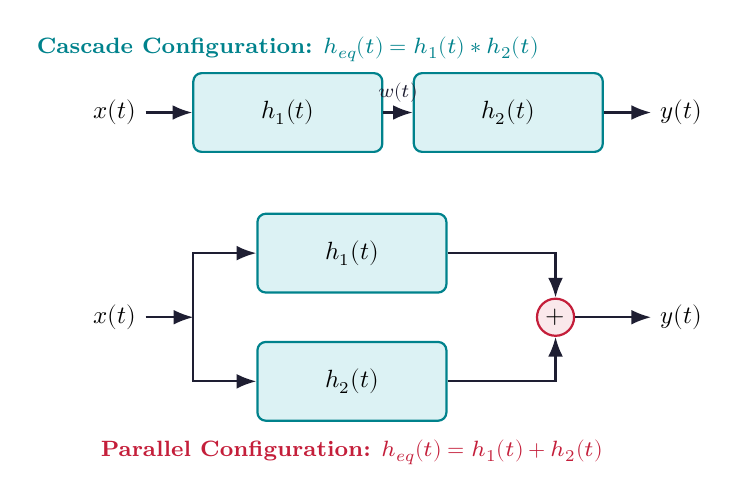
\begin{tikzpicture}[>=Latex, node distance=1.8cm, font=\small]
  % Cascade block diagram
  \node (in1) at (0, 1.8) {$x(t)$};
  \node[sysblock, right of=in1, node distance=2.2cm] (sys1) {$h_1(t)$};
  \node[sysblock, right of=sys1, node distance=2.8cm] (sys2) {$h_2(t)$};
  \node[right of=sys2, node distance=2.2cm] (out1) {$y(t)$};
  \draw[arrowline] (in1) -- (sys1);
  \draw[arrowline] (sys1) -- node[above] {\scriptsize $w(t)$} (sys2);
  \draw[arrowline] (sys2) -- (out1);
  \node[above of=sys1, node distance=0.8cm, color=myteal] {\footnotesize \textbf{Cascade Configuration:} $h_{eq}(t) = h_1(t) * h_2(t)$};

  % Parallel block diagram
  \node (in2) at (0, -0.8) {$x(t)$};
  \coordinate[right of=in2, node distance=1.0cm] (branch);
  \node[sysblock, above right=0.3cm and 0.8cm of branch] (p1) {$h_1(t)$};
  \node[sysblock, below right=0.3cm and 0.8cm of branch] (p2) {$h_2(t)$};
  \node[circnode, right of=branch, node distance=4.6cm] (sum) {$+$};
  \node[right of=sum, node distance=1.6cm] (out2) {$y(t)$};

  \draw[arrowline] (in2) -- (branch);
  \draw[arrowline] (branch) |- (p1);
  \draw[arrowline] (branch) |- (p2);
  \draw[arrowline] (p1) -| (sum);
  \draw[arrowline] (p2) -| (sum);
  \draw[arrowline] (sum) -- (out2);
  \node[below of=p2, node distance=0.9cm, color=myred] {\footnotesize \textbf{Parallel Configuration:} $h_{eq}(t) = h_1(t) + h_2(t)$};
\end{tikzpicture}
\end{center}
\end{tcolorbox}

% ───────────────────────────────────────────────────────────────────────────────
\section{Causality and Stability of LSI Systems}
% ───────────────────────────────────────────────────────────────────────────────

\subsection{Characterization of Causality}
A system is causal if the output at any instant $t_0$ depends only on the input values for $t \le t_0$.

\begin{tcolorbox}[defbox, title={\textbf{Causality Criterion for LSI Systems}}]
A continuous-time (or discrete-time) LSI system is \textbf{causal} if and only if its impulse response is zero for all negative time:
\begin{align}
  \text{CT:} \quad &h(t) = 0 \quad \forall t < 0 \\
  \text{DT:} \quad &h[n] = 0 \quad \forall n < 0
\end{align}
\end{tcolorbox}

\textbf{Proof of Causality Condition:}
The convolution integral gives:
\begin{equation}
  y(t) = \int_{-\infty}^{\infty} h(\tau) x(t - \tau) d\tau = \int_{-\infty}^0 h(\tau) x(t - \tau) d\tau + \int_0^{\infty} h(\tau) x(t - \tau) d\tau
\end{equation}
For $\tau < 0$, the term $t - \tau > t$, representing future input values. Thus, for $y(t)$ to be completely independent of future inputs $x(t - \tau)$ ($\tau < 0$), we must have:
\begin{equation}
  h(\tau) = 0 \quad \text{for all } \tau < 0
\end{equation}
Under causality, the convolution limits simplify to:
\begin{equation}
  y(t) = \int_0^{\infty} h(\tau) x(t - \tau) d\tau = \int_{-\infty}^{t} x(\tau) h(t - \tau) d\tau
\end{equation}
If the input $x(t)$ is also causal ($x(t) = 0$ for $t < 0$):
\begin{equation}
  y(t) = \int_0^t x(\tau) h(t - \tau) d\tau \quad (t \ge 0)
\end{equation}

\subsection{Characterization of BIBO Stability}
A system is Bounded-Input Bounded-Output (BIBO) stable if every bounded input $|x(t)| \le M_x < \infty$ produces a bounded output $|y(t)| \le M_y < \infty$.

\begin{tcolorbox}[formulabox, title={\textbf{BIBO Stability Criterion for LSI Systems}}]
An LSI system is \textbf{BIBO stable} if and only if its impulse response is \textbf{absolutely integrable} (in CT) or \textbf{absolutely summable} (in DT):
\begin{align}
  \text{CT:} \quad &\int_{-\infty}^{\infty} |h(t)| dt < \infty \\
  \text{DT:} \quad &\sum_{n=-\infty}^{\infty} |h[n]| < \infty
\end{align}
\end{tcolorbox}

\begin{tcolorbox}[examplebox, title={\textbf{Rigorous Proof of BIBO Stability Criterion (Sufficiency and Necessity)}}]
\textbf{1. Sufficiency Proof (If $\int |h(t)|dt < \infty \implies$ BIBO Stable):}
Let $|x(t)| \le M_x < \infty$. Taking the magnitude of the output:
\begin{align*}
  |y(t)| &= \left| \int_{-\infty}^{\infty} h(\tau) x(t - \tau) d\tau \right| \le \int_{-\infty}^{\infty} |h(\tau)| \cdot |x(t - \tau)| d\tau \\
  &\le M_x \int_{-\infty}^{\infty} |h(\tau)| d\tau
\end{align*}
Since $\int_{-\infty}^\infty |h(\tau)| d\tau = K < \infty$, we have $|y(t)| \le M_x K < \infty$ for all $t$. Hence, the output is guaranteed bounded.

\textbf{2. Necessity Proof (If BIBO Stable $\implies \int |h(t)|dt < \infty$):}
Suppose $\int_{-\infty}^\infty |h(t)|dt = \infty$. Choose the bounded input:
\begin{equation*}
  x(t - \tau) = \text{sgn}[h(\tau)] = \begin{cases} +1, & h(\tau) > 0 \\ -1, & h(\tau) < 0 \end{cases}
\end{equation*}
Clearly $|x(t)| = 1 \le 1$ is bounded. Then at time $t = 0$:
\begin{equation*}
  y(0) = \int_{-\infty}^{\infty} h(\tau) x(-\tau) d\tau = \int_{-\infty}^{\infty} h(\tau) \text{sgn}[h(\tau)] d\tau = \int_{-\infty}^{\infty} |h(\tau)| d\tau = \infty
\end{equation*}
The output grows unbounded at $t=0$, violating BIBO stability. Therefore, absolute integrability is both necessary and sufficient.
\end{tcolorbox}

% ───────────────────────────────────────────────────────────────────────────────
\section{System Representation Through Differential Equations}
% ───────────────────────────────────────────────────────────────────────────────

\subsection{Linear Constant-Coefficient Differential Equations (LCCDE)}
A continuous-time lumped parameter LTI system is generally modeled by an $N$-th order LCCDE relating input $x(t)$ to output $y(t)$:
\begin{equation}
  \sum_{k=0}^{N} a_k \frac{d^k y(t)}{dt^k} = \sum_{m=0}^{M} b_m \frac{d^m x(t)}{dt^m}
\end{equation}
where $a_k, b_m$ are real, time-invariant coefficients, and $N \ge M$ for physical realizability.

\subsection{Complete Solution: Natural and Forced Responses}
The total output consists of two components:
\begin{equation}
  y(t) = y_h(t) + y_p(t) = y_{zi}(t) + y_{zs}(t)
\end{equation}
\begin{itemize}[topsep=2pt, itemsep=2pt]
  \item \textbf{Homogeneous Solution $y_h(t)$ (Natural Response):} Solution when input $x(t) \equiv 0$:
  \begin{equation}
    \sum_{k=0}^N a_k \frac{d^k y(t)}{dt^k} = 0 \implies \sum_{k=0}^N a_k \lambda^k = 0 \quad \text{(Characteristic Equation)}
  \end{equation}
  If roots $\lambda_i$ are distinct: $y_h(t) = \sum_{i=1}^N C_i e^{\lambda_i t}$.
  \item \textbf{Particular Solution $y_p(t)$ (Forced Response):} The specific response satisfying the non-zero input excitation $x(t)$.
  \item \textbf{Zero-Input Response (ZIR) $y_{zi}(t)$:} Response produced purely by internal stored energy (initial conditions) with zero external input.
  \item \textbf{Zero-State Response (ZSR) $y_{zs}(t)$:} Response produced purely by the input with all initial conditions set to zero: $y_{zs}(t) = x(t) * h(t)$.
\end{itemize}

\subsection{Condition of Initial Rest}
\begin{tcolorbox}[defbox, title={\textbf{Concept: Initial Rest}}]
An LCCDE system is said to be at \textbf{Initial Rest} if the system starts with zero energy storage prior to input application:
\begin{equation}
  \text{If } x(t) = 0 \text{ for } t \le t_0 \implies y(t) = 0 \text{ for } t \le t_0
\end{equation}
Initial rest is the necessary and sufficient condition that guarantees the differential equation system is \textbf{Linear}, \textbf{Time-Invariant}, and \textbf{Causal}.
\end{tcolorbox}

\subsection{Block Diagram Realization of LCCDE Systems}
LCCDEs can be physically synthesized using three elementary operational building blocks:
\begin{enumerate}[topsep=2pt, itemsep=2pt]
  \item \textbf{Integrators ($\int$):} preferred over differentiators because differentiators amplify high-frequency noise.
  \item \textbf{Adders / Summers ($\sum$):} compute algebraic additions.
  \item \textbf{Scalers / Multipliers ($a_k, b_m$):} amplify signals by constant gains.
\end{enumerate}

\begin{tcolorbox}[tikzbox, title={\textbf{TikZ Schematic: Direct Form II (Canonic) Realization of 2nd-Order LCCDE}}]
\begin{center}
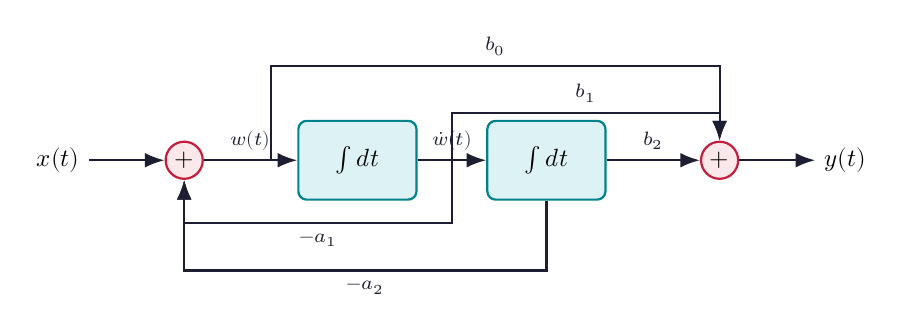
\begin{tikzpicture}[>=Latex, node distance=2cm, font=\small]
  % Input and first summer
  \node (x) at (0,0) {$x(t)$};
  \node[circnode, right of=x, node distance=1.6cm] (s1) {$+$};
  \draw[arrowline] (x) -- (s1);

  % Central integrator chain
  \node[sysblock, right of=s1, node distance=2.2cm, minimum width=1.5cm] (int1) {$\int dt$};
  \node[sysblock, right of=int1, node distance=2.4cm, minimum width=1.5cm] (int2) {$\int dt$};
  \draw[arrowline] (s1) -- node[above] {\scriptsize $w(t)$} (int1);
  \draw[arrowline] (int1) -- node[above] {\scriptsize $\dot{w}(t)$} (int2);

  % Second summer and output
  \node[circnode, right of=int2, node distance=2.2cm] (s2) {$+$};
  \node[right of=s2, node distance=1.6cm] (y) {$y(t)$};
  \draw[arrowline] (s2) -- (y);

  % Direct feedthrough
  \draw[arrowline] ($(s1)!0.5!(int1)$) -- ++(0,1.2) -| node[pos=0.25, above] {\scriptsize $b_0$} (s2);

  % Forward paths (zeros)
  \draw[arrowline] ($(int1)!0.5!(int2)$) -- ++(0,0.6) -| node[pos=0.25, above] {\scriptsize $b_1$} (s2);
  \draw[arrowline] (int2) -- node[above] {\scriptsize $b_2$} (s2);

  % Feedback paths (poles)
  \draw[arrowline] ($(int1)!0.5!(int2)$) -- ++(0,-0.8) -| node[pos=0.25, below] {\scriptsize $-a_1$} (s1);
  \draw[arrowline] (int2) -- ++(0,-1.4) -| node[pos=0.25, below] {\scriptsize $-a_2$} (s1);
\end{tikzpicture}
\end{center}
\end{tcolorbox}

% ───────────────────────────────────────────────────────────────────────────────
\section{Behavior with Aperiodic Convergent Inputs}
% ───────────────────────────────────────────────────────────────────────────────

When an aperiodic convergent input signal (such as an exponentially decaying signal $x(t) = e^{-at}u(t)$, $a > 0$) is applied to an LSI system:
\begin{itemize}[topsep=2pt, itemsep=2pt]
  \item \textbf{Energy Preservation:} If both $x(t)$ and $h(t)$ are $L_1$ and $L_2$ bounded (energy signals), the output $y(t) = x(t) * h(t)$ is also guaranteed to be an energy signal:
  \begin{equation}
    E_y = \int_{-\infty}^{\infty} |y(t)|^2 dt < \infty
  \end{equation}
  \item \textbf{Convergence to Zero:} Since $\lim_{t \to \infty} x(t) = 0$, for any stable system with $\int |h(t)|dt < \infty$, the output asymptotically decays to zero:
  \begin{equation}
    \lim_{t \to \infty} y(t) = \lim_{t \to \infty} \int_0^t x(\tau) h(t - \tau) d\tau = 0
  \end{equation}
  \item \textbf{Transient Decay Rate:} The overall decay envelope is governed by the slowest pole (dominant time constant) among the system and the input excitation.
\end{itemize}

% ───────────────────────────────────────────────────────────────────────────────
% QUICK REVISION PAGE
% ───────────────────────────────────────────────────────────────────────────────
\newpage
\begin{center}
  {\Large\bfseries\color{myred} Quick Revision \& Examination Compendium}\\[3pt]
  {\small\color{watermark}\textbf{Module 2: Linear Shift-Invariant Systems \& Convolution}}
\end{center}
\vspace{-2pt}
\noindent{\color{myred}\rule{\linewidth}{0.8pt}}

\begin{tcolorbox}[formulabox, title={\textbf{Key Formulas at a Glance}}]
\par\vspace{4pt}\noindent
\begingroup
\setlength{\tabcolsep}{5pt}
\setlength{\extrarowheight}{3pt}
\renewcommand{\arraystretch}{1.4}
\begin{tabularx}{\linewidth}{|B{4.5cm}|Y|}
\hline
\textbf{Concept / Law} & \textbf{Mathematical Equation} \\
\hline
Continuous-Time Convolution & $y(t) = x(t) * h(t) = \int_{-\infty}^{\infty} x(\tau) h(t - \tau) d\tau$ \\
\hline
Discrete-Time Convolution & $y[n] = x[n] * h[n] = \sum_{k=-\infty}^{\infty} x[k] h[n - k]$ \\
\hline
Step Response from Impulse & $s(t) = \int_{-\infty}^t h(\tau) d\tau, \quad s[n] = \sum_{k=-\infty}^n h[k]$ \\
\hline
Impulse Response from Step & $h(t) = \frac{ds(t)}{dt}, \quad h[n] = s[n] - s[n-1]$ \\
\hline
LTI Causality Condition & $h(t) = 0 \quad \forall t < 0, \qquad h[n] = 0 \quad \forall n < 0$ \\
\hline
LTI BIBO Stability Condition & $\int_{-\infty}^{\infty} |h(t)| dt < \infty, \qquad \sum_{n=-\infty}^{\infty} |h[n]| < \infty$ \\
\hline
Cascade Connection & $h_{eq}(t) = h_1(t) * h_2(t) = h_2(t) * h_1(t)$ \\
\hline
Parallel Connection & $h_{eq}(t) = h_1(t) + h_2(t)$ \\
\hline
Convolution with Shifted Impulse & $x(t) * \delta(t - t_0) = x(t - t_0)$ \\
\hline
LCCDE Zero-State Output & $y_{zs}(t) = x(t) * h(t) \quad \text{under initial rest}$ \\
\hline
\end{tabularx}
\endgroup
\end{tcolorbox}

\begin{tcolorbox}[defbox, title={\textbf{One-Line Definitions for Rapid Review}}]
\par\vspace{4pt}\noindent
\begingroup
\setlength{\tabcolsep}{5pt}
\setlength{\extrarowheight}{3pt}
\renewcommand{\arraystretch}{1.35}
\begin{tabularx}{\linewidth}{|B{4.2cm}|Y|}
\hline
\textbf{Term} & \textbf{Definitive Technical Meaning} \\
\hline
Impulse Response $h(t)$ & The output response of an LTI system when excited by a unit impulse under zero initial conditions. \\
\hline
Step Response $s(t)$ & The response of an LTI system to a unit step input under initial rest conditions. \\
\hline
Convolution & A mathematical operator combining two signals to express how the shape of one is modified by the other. \\
\hline
Initial Rest & The condition where a system has zero internal energy stored prior to the instant an input is applied. \\
\hline
Causal LSI System & An LTI system whose impulse response is strictly zero for all negative time ($h(t) = 0, t < 0$). \\
\hline
BIBO Stable LSI System & An LTI system whose impulse response is absolutely integrable ($\int |h(t)|dt < \infty$). \\
\hline
Zero-Input Response (ZIR) & The system output generated solely by non-zero initial states in the absence of any input. \\
\hline
Zero-State Response (ZSR) & The system output generated solely by the external input when all initial states are zero. \\
\hline
Canonic Realization & A block diagram realization containing the minimum possible number of delay or integrator elements ($N$). \\
\hline
\end{tabularx}
\endgroup
\end{tcolorbox}

\begin{tcolorbox}[exambox, title={\textbf{Frequently Asked / Viva Questions}}]
\begin{enumerate}[topsep=0pt, label=\textbf{Q\arabic*.}, itemsep=5pt]
  \item \Q{Why does the impulse response $h(t)$ completely characterize an LSI system?}
  Because any input $x(t)$ can be represented as an integral of weighted, shifted impulses. By linearity (superposition) and time-invariance, the output is the corresponding integral of weighted, shifted impulse responses. Thus, knowing $h(t)$ determines the response to \textit{any} arbitrary input.

  \item \Q{How can you compute the impulse response if the step response is known?}
  For continuous-time systems, differentiate the step response: $h(t) = \frac{ds(t)}{dt}$. For discrete-time systems, take the first backward difference: $h[n] = s[n] - s[n-1]$.

  \item \Q{Prove that convolution is commutative: $x(t) * h(t) = h(t) * x(t)$.}
  By definition, $x(t) * h(t) = \int_{-\infty}^{\infty} x(\tau) h(t - \tau) d\tau$. Substituting $v = t - \tau \implies d\tau = -dv$. When $\tau = -\infty, v = +\infty$; when $\tau = +\infty, v = -\infty$. Thus:
  $\int_{+\infty}^{-\infty} x(t - v) h(v) (-dv) = \int_{-\infty}^{\infty} h(v) x(t - v) dv = h(t) * x(t)$.

  \item \Q{What is the total duration of the convolution of two signals of lengths $T_1$ and $T_2$?}
  In continuous-time, the duration is $T_1 + T_2$. In discrete-time, if signal 1 has $N_1$ samples and signal 2 has $N_2$ samples, the convolved output has exactly $N_1 + N_2 - 1$ samples.

  \item \Q{State the necessary and sufficient condition for an LSI system to be causal.}
  The impulse response must be zero for all negative time: $h(t) = 0$ for $t < 0$ (or $h[n] = 0$ for $n < 0$).

  \item \Q{Is the system with impulse response $h(t) = e^{2t} u(t)$ stable? Why?}
  No. Evaluating absolute integrability: $\int_{-\infty}^\infty |h(t)|dt = \int_0^\infty e^{2t} dt = \left[\frac{e^{2t}}{2}\right]_0^\infty = \infty$. Since it is not absolutely integrable, it is BIBO unstable.

  \item \Q{What is the difference between Zero-Input Response (ZIR) and Zero-State Response (ZSR)?}
  ZIR is driven purely by initial energy/conditions stored in capacitors/inductors with zero external input. ZSR is driven purely by the applied input with zero initial stored energy. Total response is $y(t) = y_{zir}(t) + y_{zsr}(t)$.

  \item \Q{Why does the condition of initial rest ensure that a differential equation represents an LTI system?}
  Non-zero initial conditions introduce an additive constant independent of the input, violating linearity (homogeneity $y(0) \ne 0$) and causing time-variant behavior. Initial rest enforces zero state prior to excitation, ensuring linearity, time-invariance, and causality.

  \item \Q{Why are integrators preferred over differentiators in analog computer simulation of LCCDE?}
  Differentiators have transfer function $s$, which amplifies high-frequency noise and introduces signal instability. Integrators have transfer function $1/s$, which attenuates high frequencies, acting as low-pass filters that provide stable, noise-free computation.

  \item \Q{What is the convolution of a signal $x(t)$ with a unit step $u(t)$?}
  $x(t) * u(t) = \int_{-\infty}^\infty x(\tau) u(t - \tau) d\tau = \int_{-\infty}^t x(\tau) d\tau$. Convolution with a unit step is equivalent to running integration of the signal from $-\infty$ to $t$.
\end{enumerate}
\end{tcolorbox}

\begin{tcolorbox}[tikzbox, title={\textbf{Summary Matrix: LSI Characterization Across Domains}}]
\par\vspace{4pt}\noindent
\begingroup
\setlength{\tabcolsep}{4.5pt}
\setlength{\extrarowheight}{3pt}
\renewcommand{\arraystretch}{1.35}
\begin{tabularx}{\linewidth}{|B{3.2cm}|B{4.5cm}|Y|}
\hline
\textbf{Property} & \textbf{Continuous-Time (CT)} & \textbf{Discrete-Time (DT)} \\
\hline
Impulse Input & Dirac Delta $\delta(t)$ & Kronecker Delta $\delta[n]$ \\
\hline
Convolution & $y(t) = \int_{-\infty}^\infty x(\tau) h(t-\tau) d\tau$ & $y[n] = \sum_{k=-\infty}^\infty x[k] h[n-k]$ \\
\hline
Causality & $h(t) = 0 \quad \forall t < 0$ & $h[n] = 0 \quad \forall n < 0$ \\
\hline
BIBO Stability & $\int_{-\infty}^\infty |h(t)| dt < \infty$ & $\sum_{n=-\infty}^\infty |h[n]| < \infty$ \\
\hline
Step Response $s$ & $s(t) = \int_{-\infty}^t h(\tau) d\tau$ & $s[n] = \sum_{k=-\infty}^n h[k]$ \\
\hline
Recovery of $h$ & $h(t) = \frac{ds(t)}{dt}$ & $h[n] = s[n] - s[n-1]$ \\
\hline
Interconnection & Cascade: $h_1 * h_2$; Parallel: $h_1 + h_2$ & Cascade: $h_1 * h_2$; Parallel: $h_1 + h_2$ \\
\hline
\end{tabularx}
\endgroup
\end{tcolorbox}

\end{document}
